\documentclass[twocolumn, 11pt]{article}

\usepackage[a4paper,margin=2cm]{geometry}
\usepackage{soul, color}
\usepackage{hyperref}
\usepackage[australian]{babel}
\usepackage{graphicx}
\usepackage{csquotes}
\usepackage[backend=biber,dateabbrev=false]{biblatex}
\usepackage{fancyvrb}
\usepackage{booktabs}
\usepackage{float}
\usepackage{subcaption}

\addbibresource{references.bib}

\title{COMP30027 Assignment 2 - Report}
\date{\today}
\author{\textbf{Anonymous}}

\VerbatimFootnotes

\begin{document}
\maketitle
This task involved classifying recipes according to their duration, based on the recipe name, ingredients, steps, number of steps, and number of ingredients. Each recipe originated from one of three classes; \verb|short|, \verb|medium| or \verb|long|, which were encoded as \verb|1.0|, \verb|2.0| and \verb|3.0| respectively.\\[2mm]
The dataset is provided courtesy of \textit{Shuyang Li et. al.} \cite{majumder2019generating}, who scraped the recipe data from \url{food.com}. 40,000 labelled training instances were provided, and accuracies presented in this report were generated from the public Kaggle competition, for which 10,000 predictions were submitted and 3,000 were assessed for accuracy.
\section{Classifiers}
\subsection{Support Vector Classifier}
\label{sec: SVC}
A Support Vector Classifier (SVC) using a Radial Basis Function (RBF) was implemented with \textit{Scikit-learn} \cite{scikit-learn}. The RBF kernel was used since it is relatively simple to tune the hyperparameters of the model and achieve good performance. After tuning, an ultimate value of $C=1$ was reached, and the performance of the SVC with the RBF was superior to linear and polynomial kernels.\\[2mm]
This classifier used the provided \verb|doc2vec100| datasets, which were concatenated, and the extra numeric features were standardised, then added as additional attributes to produce a 203-dimensional dataset.

\subsection{Gaussian Naïve Bayes Ensemble}
As an alternative and experimental model, an ensemble was composed out of 5 unique Gaussian Naïve Bayes (GNB) \cite{scikit-learn} classifiers. For the training data of these classifiers the entire training set was partitioned by its 5 columns, each partition containing a single attribute of the original dataset. This was motivated out curiosity for what would happen if an ensemble model was generated by partitioning over the features instead of instances, as this was found rarely in literature.\\[2mm]
So that GNB classifiers would be compatible with each of these datasets the count vectorized data was used for each of the textual features, and the numeric features were taken directly.\\[2mm]
After training they were combined into an ensemble model through simple voting, which was implemented manually due to the assumption made by \textit{Scikit-learn's} \verb|VotingClassifier| that all models are trained on identical training data \footnote{MLxtend's \verb|EnsembleVoteClassifier| also supports this vertical feature partitioning \url{http://rasbt.github.io/mlxtend/}}.

\subsection{Convolutional Neural Network} 
The final model generated was a sequential Convolutional Neural Network, implemented with \textit{Keras} \cite{chollet2015keras} and \textit{TensorFlow} \cite{tensorflow2015}.\\[2mm]
As input, this model takes a string containing all columns of the training data present in the CSV. The first layer of the model then vectorizes this input into a length 300 tensor of integers, then passes the numeric vector to an embedding layer, which produces a 128-dimensional representation of each word. Groups of 5 of these embeddings are passed into a convolutional layer, then max-pooling is applied, and finally a dense layer is used to generate the final classifications. A diagram of this neural network architecture is included as Figure \ref{fig: NN architecture}.
% The network was trained for only 3 epochs over the training data since the validation loss increased significantly when more training was performed. It is likely that the network trained successfully in so few instances because of the relatively small dimension of the output space (3 classes.)
\begin{figure*}[!ht]
    \centering
    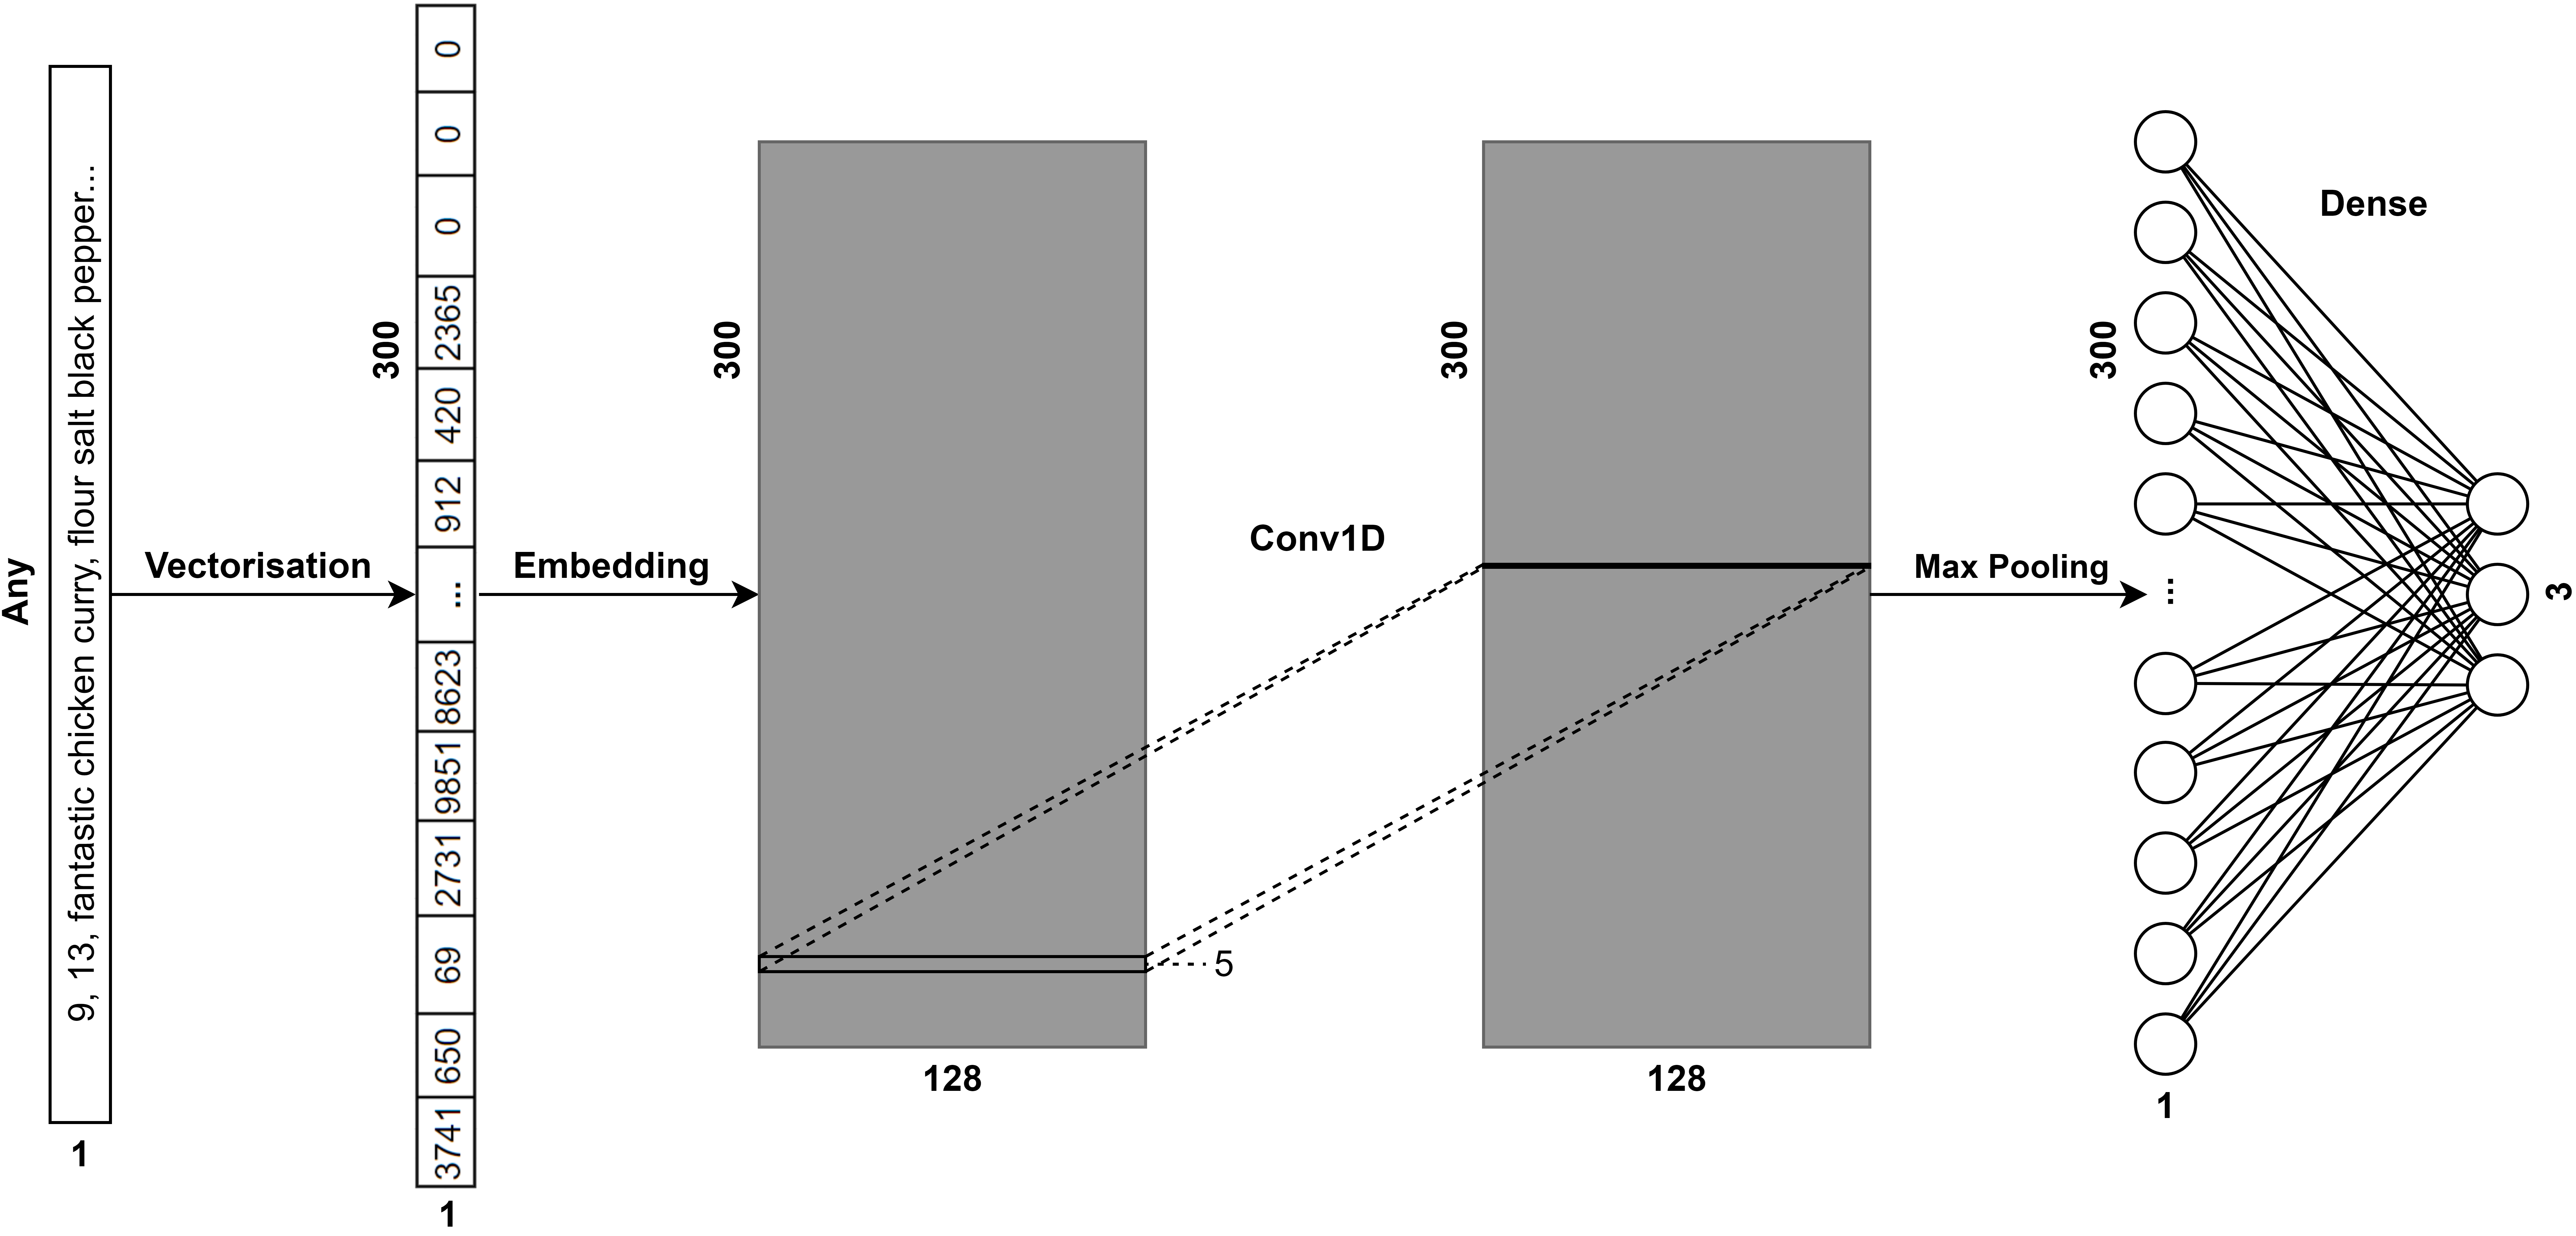
\includegraphics[width=\textwidth]{architecture.png}
    \caption{The Architecture used in the Convolutional Neural Network Classifier.}
    \label{fig: NN architecture}
\end{figure*}
\section{Evaluation}
\subsection{Support Vector Classifier}
In training, this classifier used the provided \verb|doc2vec100| dataset since this performed better than the \verb|doc2vec50| instances. This is because SVCs do not suffer from the curse of dimensionality, so it is likely that in the 100 dimensional space the SVC has an easier time generating a decision boundary due to the increased amount of attributes which it could use to differentiate instances.\\[2mm]
This model performed with 72.37\% accuracy on the public Kaggle competition, outperforming a SVC trained on identical data but using a linear kernel by 0.87\%. The precision and recall statistics for the model are provided in Tables \ref{tab: precision} \& \ref{tab: recall}.

\subsection{Gaussian Naïve Bayes Ensemble}
Tested against an isolated split of the training data, each of the 5 GNB models which comprise the ensemble scored as shown in Table \ref{tab: GNB scores}.
\begin{table}[H]
    \centering
    \begin{tabular}{@{}lll@{}}
    \toprule
    Feature               & Data Type & Accuracy \\ \midrule
    names                 & \verb|doc2vec|   & 0.4197   \\
    steps                 & \verb|doc2vec|   & 0.4033   \\
    ingredients           & \verb|doc2vec|   & 0.1893   \\
    number of steps       & \verb|int|       & 0.5948   \\
    number of ingredients & \verb|int|       & 0.6026   \\ \bottomrule
    \end{tabular}
    \caption{Accuracies of the Individual GNB Models}
    \label{tab: GNB scores}
\end{table}
The reasoning for these scores is discussed further in section \ref{sec: Discussion}.\\[2mm]
When combined with equal weight voting, the model achieves an accuracy of 56.62\%. But since it would therefore be more accurate to simply use either one of the integer models, weighted voting was implemented.\\[2mm]
Since the accuracies of the models were approximately at a ratio of \verb|2:2:1:3:3| these were the first weights implemented in the voting system. After testing a variety of alternatives this ultimately provided the highest level of ensemble accuracy, slightly better than any of the individual models at 62.33\%.

\subsection{Convolutional Neural Network}
The CNN had the best performance out of all the classifiers. It achieved an accuracy of 81.83\% on the public subset of the test data. This is an improvement of 9.46\% over the SVC, and is 19.50\% better than the GNB ensemble.

\subsection{Precision and Recall}
Generally these statistics are as could be expected, however it is somewhat surprising that both the precision and recall of the GNB classifier on class \verb|3.0| are so poor. This indicates that it was not only predicting class \verb|3.0| for many instances of other classes, but also that it was missing the true class \verb|3.0| instances most of the time.
\begin{table}[!h]
    \centering
    \begin{tabular}{@{}llll@{}}
    \toprule
    Classifier & \verb|1.0| & \verb|2.0| & \verb|3.0| \\ \midrule
    SVC                            & 70.0\%                    & 74.2\%                    & 35.5\%                    \\
    GNB ensemble                   & 79.4\%                    & 49.2\%                    & 43.5\%                    \\
    CNN                            & 80.7\%                    & 83.7\%                    & 68.3\%                    \\ \bottomrule
    \end{tabular}
    \caption{Precision for Each of the Classifiers and Classes}
    \label{tab: precision}
\end{table}
\begin{table}[!h]
    \centering
    \begin{tabular}{@{}llll@{}}
    \toprule
    Classifier & \verb|1.0| & \verb|2.0| & \verb|3.0| \\ \midrule
    SVC          & 69.4\%                    & 71.4\%                    & 65.4\%                    \\
    GNB ensemble & 61.2\%                    & 78.2\%                    & 21.0\%                    \\
    CNN          & 81.5\%                    & 82.6\%                    & 72.0\%                    \\ \bottomrule
    \end{tabular}
    \caption{Recall for Each of the Classifiers and Classes}
    \label{tab: recall}
\end{table}
\section{Discussion and Error Analysis}
\label{sec: Discussion}
\textbf{Gaussian Naïve Bayes} makes the assumption that features are independent, and that instances are normally distributed within each class. To see how these assumptions are violated, consider the text based attributes, the names, steps, and ingredients. By projecting the 100-dimensional text vectorisation space down into 2 dimensions it is possible to visualise the distribution of a sample of this data \cite{rehurek_lrec}. Such a visualisation is shown in Figure \ref{fig: doc2vec}, where it is clear that the vectorized words from the recipe dataset form an annulus shape.\\[2mm]
From this distribution it is clear that the instances violate the assumption of normality within each class. It is also clear that the independence assumption is violated, as there is a clear correlation between these points.\\[2mm]
The assumption of normality is more reasonable for the numeric attributes, which is why these see significantly better performance and are represented more favourably in the weighted ensemble model, however strong correlation can be observed between the number of ingredients and steps. All of these violations contribute to the poor performance of the GNB ensemble.\\[2mm]
The \textbf{Support Vector Classifier} performed significantly better at the classification task. As mentioned in section \ref{sec: SVC} this is due to it's ability to work effectively with high-dimensional data. After experimentation with a range of values for $C$, the regularisation parameter, a value of 1 was selected. This moderate value is reasonable considering the high dimension of the feature space, since in the high dimensional space the model finds it easier to create boundaries between classes, and therefore does not require the softer margins afforded by smaller values of $C$.\\[2mm]
Finally, the \textbf{Convolutional Neural Network} which performed significantly better than both aforementioned models. It is believed that the CNN classifier is able to achieve this performance due to its use of both embedding and convolutional layers.\\[2mm]
Although the single convolutional layer in the model is only capable of learning linear decision boundaries on its input, it is important to realise that the input to the convolutional layer is not a direct vectorisation of the text data. Instead, the vectorized text is passed through an embedding layer, which transforms the data into a 128-dimensional embedding space. This introduces non-linearity into the model, and since the embedding is designed to place related words nearby in the embedding space, the single convolutional layer is able to form linear boundaries in this space which differentiate classes effectively.\\[2mm]
When training the CNN, out of the 40,000 training instances, 10\% were reserved for testing, and of the remaining 36,000 20\% (7,200) were reserved for validation. The other 28,800 were used to train the model. The training duration was determined by the amount of epochs required before the validation loss begun to increase, which resulted in a training time of 3 epochs. A visualisation of the training and validation accuracies and losses which shows this appears in Figure \ref{fig: NN stats}.
\printbibliography
\newpage
\onecolumn
\null
\vfill
\begin{figure}[ht]
    \centering
    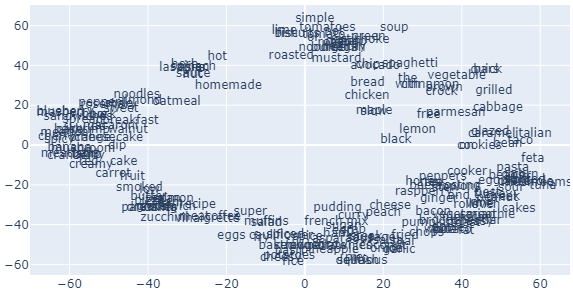
\includegraphics[width=0.9\textwidth]{doc2vec-visualisation.png}
    \caption{A 2D Projection of the Distribution of 200 Words in the 100-dimensional doc2vec Space.}
    \label{fig: doc2vec}
\end{figure}
\vfill
\begin{figure}[hb]
    \centering
    \begin{subfigure}[b]{0.45\linewidth}
        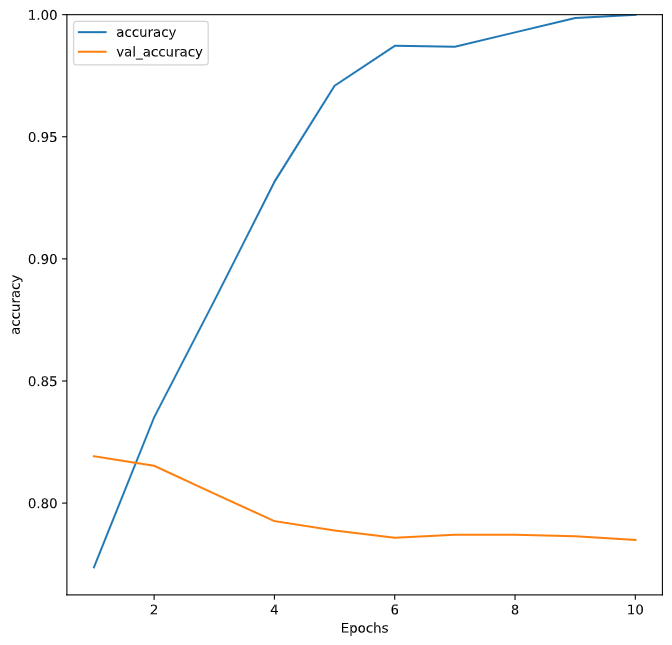
\includegraphics[width=\linewidth]{NN-acc.png}
        \caption{Accuracies}
        \label{fig: NN acc}
    \end{subfigure}
    \begin{subfigure}[b]{0.45\linewidth}
        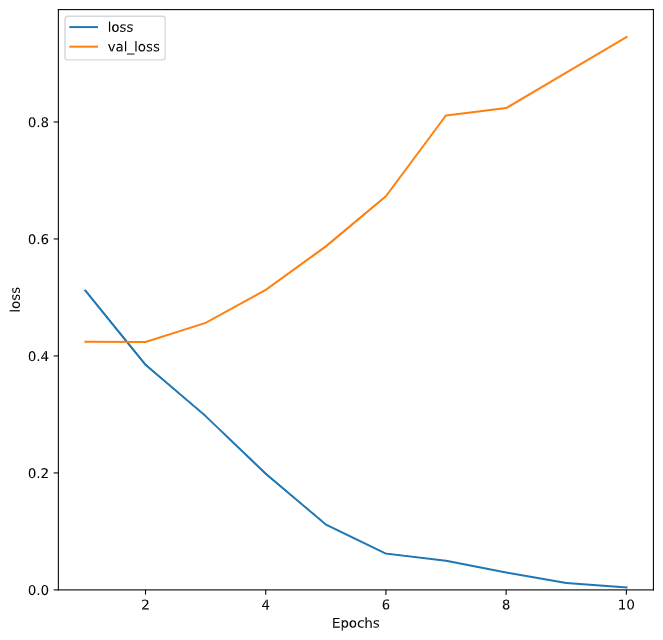
\includegraphics[width=\linewidth]{NN-loss.png}
        \caption{Losses}
        \label{fig: NN loss}
    \end{subfigure}
    \caption{CNN Training and Validation Statistics}
    \label{fig: NN stats}
\end{figure}
\vfill



\end{document}